\documentclass[11pt,oneside]{amsart}
\usepackage{geometry}
\usepackage{amssymb,parskip,mathtools,microtype}
\usepackage[shortlabels]{enumitem}
\usepackage[most]{tcolorbox}

\definecolor{sol}{rgb}{0.1, 0.3, 0.6}

\newtcolorbox{solution}{enhanced, breakable, colframe=sol, title=Solution}

\theoremstyle{definition}
\newtheorem{problem}{Problem}

\newcommand{\bC}{\mathbb{C}}
\newcommand{\bQ}{\mathbb{Q}}
\newcommand{\bR}{\mathbb{R}}
\newcommand{\bZ}{\mathbb{Z}}

\title{MATH1103 Fall 2022\\
Problem Set 1}

\begin{document}
    \maketitle
    This problem set is due on Wednesday, September 7 at 11:59 pm. Each problem part is worth 3 points. Collaboration is encouraged. In all cases, you must write your own solutions, and and you must cite collaborators and resources used.

    \begin{problem}
        Algebra, functions, and differential calculus review and practice.
        \begin{enumerate}[(a)]
            % \item What is $\sqrt{20}+\sqrt{45}$?
            \item Find a clever and simple way to evaluate $1002\cdot 998$.
            \begin{solution}
                The pattern here is difference of squares: $a^2-b^2=(a+b)(a-b)$, but applied in reverse!
                
                $1002\cdot 998=(1000+2)(1000-2)=1000^2-4=1000000-4=999996$.
            \end{solution}
            \item Derive a formula for $1+2+\cdots+n$, the sum of the first $n$ positive integers. Try to think of as short a derivation as possible.
            \begin{solution}
                The formula is $n(n+1)/2$. Here is my derivation and likely Gauss's original derivation as well; there are other derivations possible.
                
                If you write the sum backwards and add it to the original sum, you can group the terms as
                \[(1+n)+(2+(n-1))+(3+(n-2))+\cdots+(n+1)\]
                which is just a sum of $n$ copies of $n+1$, i.e. $n(n+1)$. So twice the sum of the first $n$ positive integers is $n(n+1)$, so the sum of the first $n$ positive integers is $n(n+1)/2$.

                Here's another derivation: If $n$ is even, we can pair up terms at opposite ends for $n/2$ pairs, each of which adds to $n+1$. Hence the sum is $n(n+1)/2$. If $n$ is odd, we can pair up terms at opposite ends, except for the term in the middle. There will be $(n-1)/2$ pairs, each summing to $n+1$, plus the lone $(n+1)/2$ in the middle. The total sum is $(n-1)(n+1)/2+(n+1)/2=n(n+1)/2$.
            \end{solution}
            \item What is $\cfrac 1{1+\cfrac 1{1+\cfrac 1{1+\cdots}}}$?
            
            You do not have to prove this continued fraction converges; just use algebra to find its value.
            \begin{solution}
                Let $x=\cfrac 1{1+\cfrac 1{1+\cfrac 1{1+\cdots}}}$. Then notice that the continued fraction can be written as
                \[\cfrac 1{1+\cfrac 1{1+\cfrac 1{1+\cdots}}}=\frac 1{1+x},\]
                so the number $x$ satisfies the equation
                \[x=\frac 1{1+x}.\]
                Solving this equation by multiplying both sides by $(1+x)$ and moving all the terms to one side, we get the quadratic
                \[x^2+x-1=0.\]
                By the quadratic formula the solutions are
                \[\frac{-1\pm\sqrt 5}2.\]
                The negative solution is clearly not the correct value of $x$ as the original fraction is visibly positive. Hence
                \[x=\frac{-1+\sqrt 5}2\approx 0.618.\]
                Fun fact: $\frac{-1+\sqrt 5}2\approx 0.618$ is the reciprocal of the golden ratio. The golden ratio itself is approximately $1.618$!

                \emph{Remark}: Alternative way to obtain the quadratic: Notice that if you take the reciprocal of $x$ and subtract 1, you get back $x$ again. In mathematical notation this says that
                \[\frac 1x-1=x.\]
                This gives the same quadratic equation $x^2+x-1=0$.
            \end{solution}
            \item What is the coefficient of $xyz$ in $(x+y+z)^3$?
            \begin{solution}
                Of course you can expand the whole thing out. You should get a lot of terms. Here's the clever way to reason about it. The product
                \[(x+y+z)(x+y+z)(x+y+z)\]
                is the sum of all possible products of a term from the first factor, a term from the second factor, and a term from the third factor. A $xyz$ term is formed by choosing any term in the first factor (3 choices), then a distinct term in the second factor (2 choices), followed by the only remaining distinct term in the third factor (1 choice). For example, we could pick $x$ then $y$ then $z$, or we could pick $y$ then $x$ then $z$, and so on. Therefore there are $3\times 2\times 1=6$ ways to form an $xyz$ term, so the coefficient of $xyz$ is 6.

                This is the same reasoning as the fact that there are 6 ways to arrange 3 people in a line. The number 6 is equal to 3 factorial!
            \end{solution}
            % \item Suppose you can take for granted that all square roots of integers which are not perfect squares are irrational. Use this to prove that $\sqrt2+\sqrt3$ is irrational.
            
            % Hint: If $\sqrt2+\sqrt3$ is rational, then its square should be rational too.
            % \item An odd (real-valued) function is defined to be a function $f\colon\bR\to\bR$ such that $f(-x)=-f(x)$ for all $x\in\bR$. An even function is defined to be a function $f\colon\bR\to\bR$ such that $f(-x)=f(x)$ for all $x\in\bR$. Prove that the product of two odd functions is an even function.
            \item Find three different real-valued functions $f$ such that $(f(x))^2=x^2$ for all $x\in\bR$.
            \begin{solution}
                A non-exhaustive list:
                \begin{itemize}
                    \item $f(x)=x$.
                    \item $f(x)=-x$.
                    \item $f(x)=|x|$.
                    \item $f(x)=-|x|$.
                    \item $f(x)=\begin{cases} x&x>1\\ -x & x\leq -1.\end{cases}$
                    \item $f(x)=\begin{cases} x&\text{$x$ is rational}\\ -x & \text{$x$ is irrational}.\end{cases}$
                    \item etc\dots
                \end{itemize}
                The principle behind this is that for every $x\in\bR$, we can choose $f(x)$ to be $x$ or $-x$, and this choice can be made independently of all other $x\in\bR$. Indeed, that's exactly the condition says. If $f$ has to be continuous, then only $x,-x,|x|,-|x|$ work. But if $f$ doesn't have to be continuous, then
                \[f(x)=\begin{cases} x&x\in A\\ -x &x\notin A\end{cases}\]
                works for any subset $A$ of $\bR$. This general example encompasses the first 4 examples: they correspond to $A=\bR,A=\varnothing,A=\bR_{\geq 0}$, and $A=\bR_{\leq 0}$ respectively. This is the most general example!
            \end{solution}
            \item State the intermediate value theorem as precisely as possible, but in your own words.
            \begin{solution}
                Example statement in my own words: The intermediate value theorem states that for any continuous function $f$ on an interval $[a,b]$, if two numbers $r$ and $s$ are in the range of $f$, then so are all the numbers in between $r$ and $s$.
            \end{solution}
            % \item Building on the previous part, prove that the derivative of an odd differentiable function is an even function.
            % \item Come up with an example of a function which is once differentiable but not twice differentiable. Show that your example works.
            \item Find a formula, in terms of the positive integer $n$, for the $n$th derivative of $\ln(x)$.
            \begin{solution}
                Let's list the first few derivatives:
                \begin{align*}
                    \frac d{dx}\ln(x) &=\frac 1x,\\
                    \frac{d^2}{dx^2}\ln(x) &= -\frac 1{x^2},\\
                    \frac{d^3}{dx^3}\ln(x) &= \frac 2{x^3},\\
                    \frac{d^4}{dx^4}\ln(x) &= -\frac 6{x^4}.
                \end{align*}
                The pattern looks like the $n$th derivative of $\ln(x)$ will be $(-1)^{n-1}\frac{(n-1)!}{x^n}$. Let's prove this by induction. The base case $n=1$ checks out since $(-1)^{1-1}(1-1)!/x^1=\frac 1x$. Now suppose we have proven that the $k$th derivative of $\ln(x)$ is equal to $(-1)^{k-1}(k-1)!/x^k$. Then the $(k+1)$th derivative of $\ln(x)$ is
                \begin{align*}
                    \frac{d^{k+1}}{dx^{k+1}}\ln(x) &= \frac d{dx}\left((-1)^{k-1}\frac{(k-1)!}{x^k}\right)\\
                    &= (-1)^{k-1}(k-1)!\frac d{dx}\left(\frac1{x^k}\right)\\
                    &= (-1)^{k-1}(k-1)!\frac{-k}{x^{k+1}}\\
                    &= (-1)^k \frac{k!}{x^{k+1}}
                \end{align*}
                which completes the induction.

                \emph{Remark}: Don't worry about the proof by mathematical induction if you have not learned how to do it. Since this class does not cover mathematical induction, finding the pattern in this case is enough.
            \end{solution}
        \end{enumerate}
    \end{problem}

    \begin{problem}
        Using only Euclidean geometry (no trigonometry), determine the area of a regular 12-sided polygon inscribed in a unit circle (i.e.\ a circle of radius 1). You should be able to get an exact answer. How close is the area to $\pi$?
    \end{problem}
    \begin{solution}
        Consider the following diagram.
        \begin{center}
        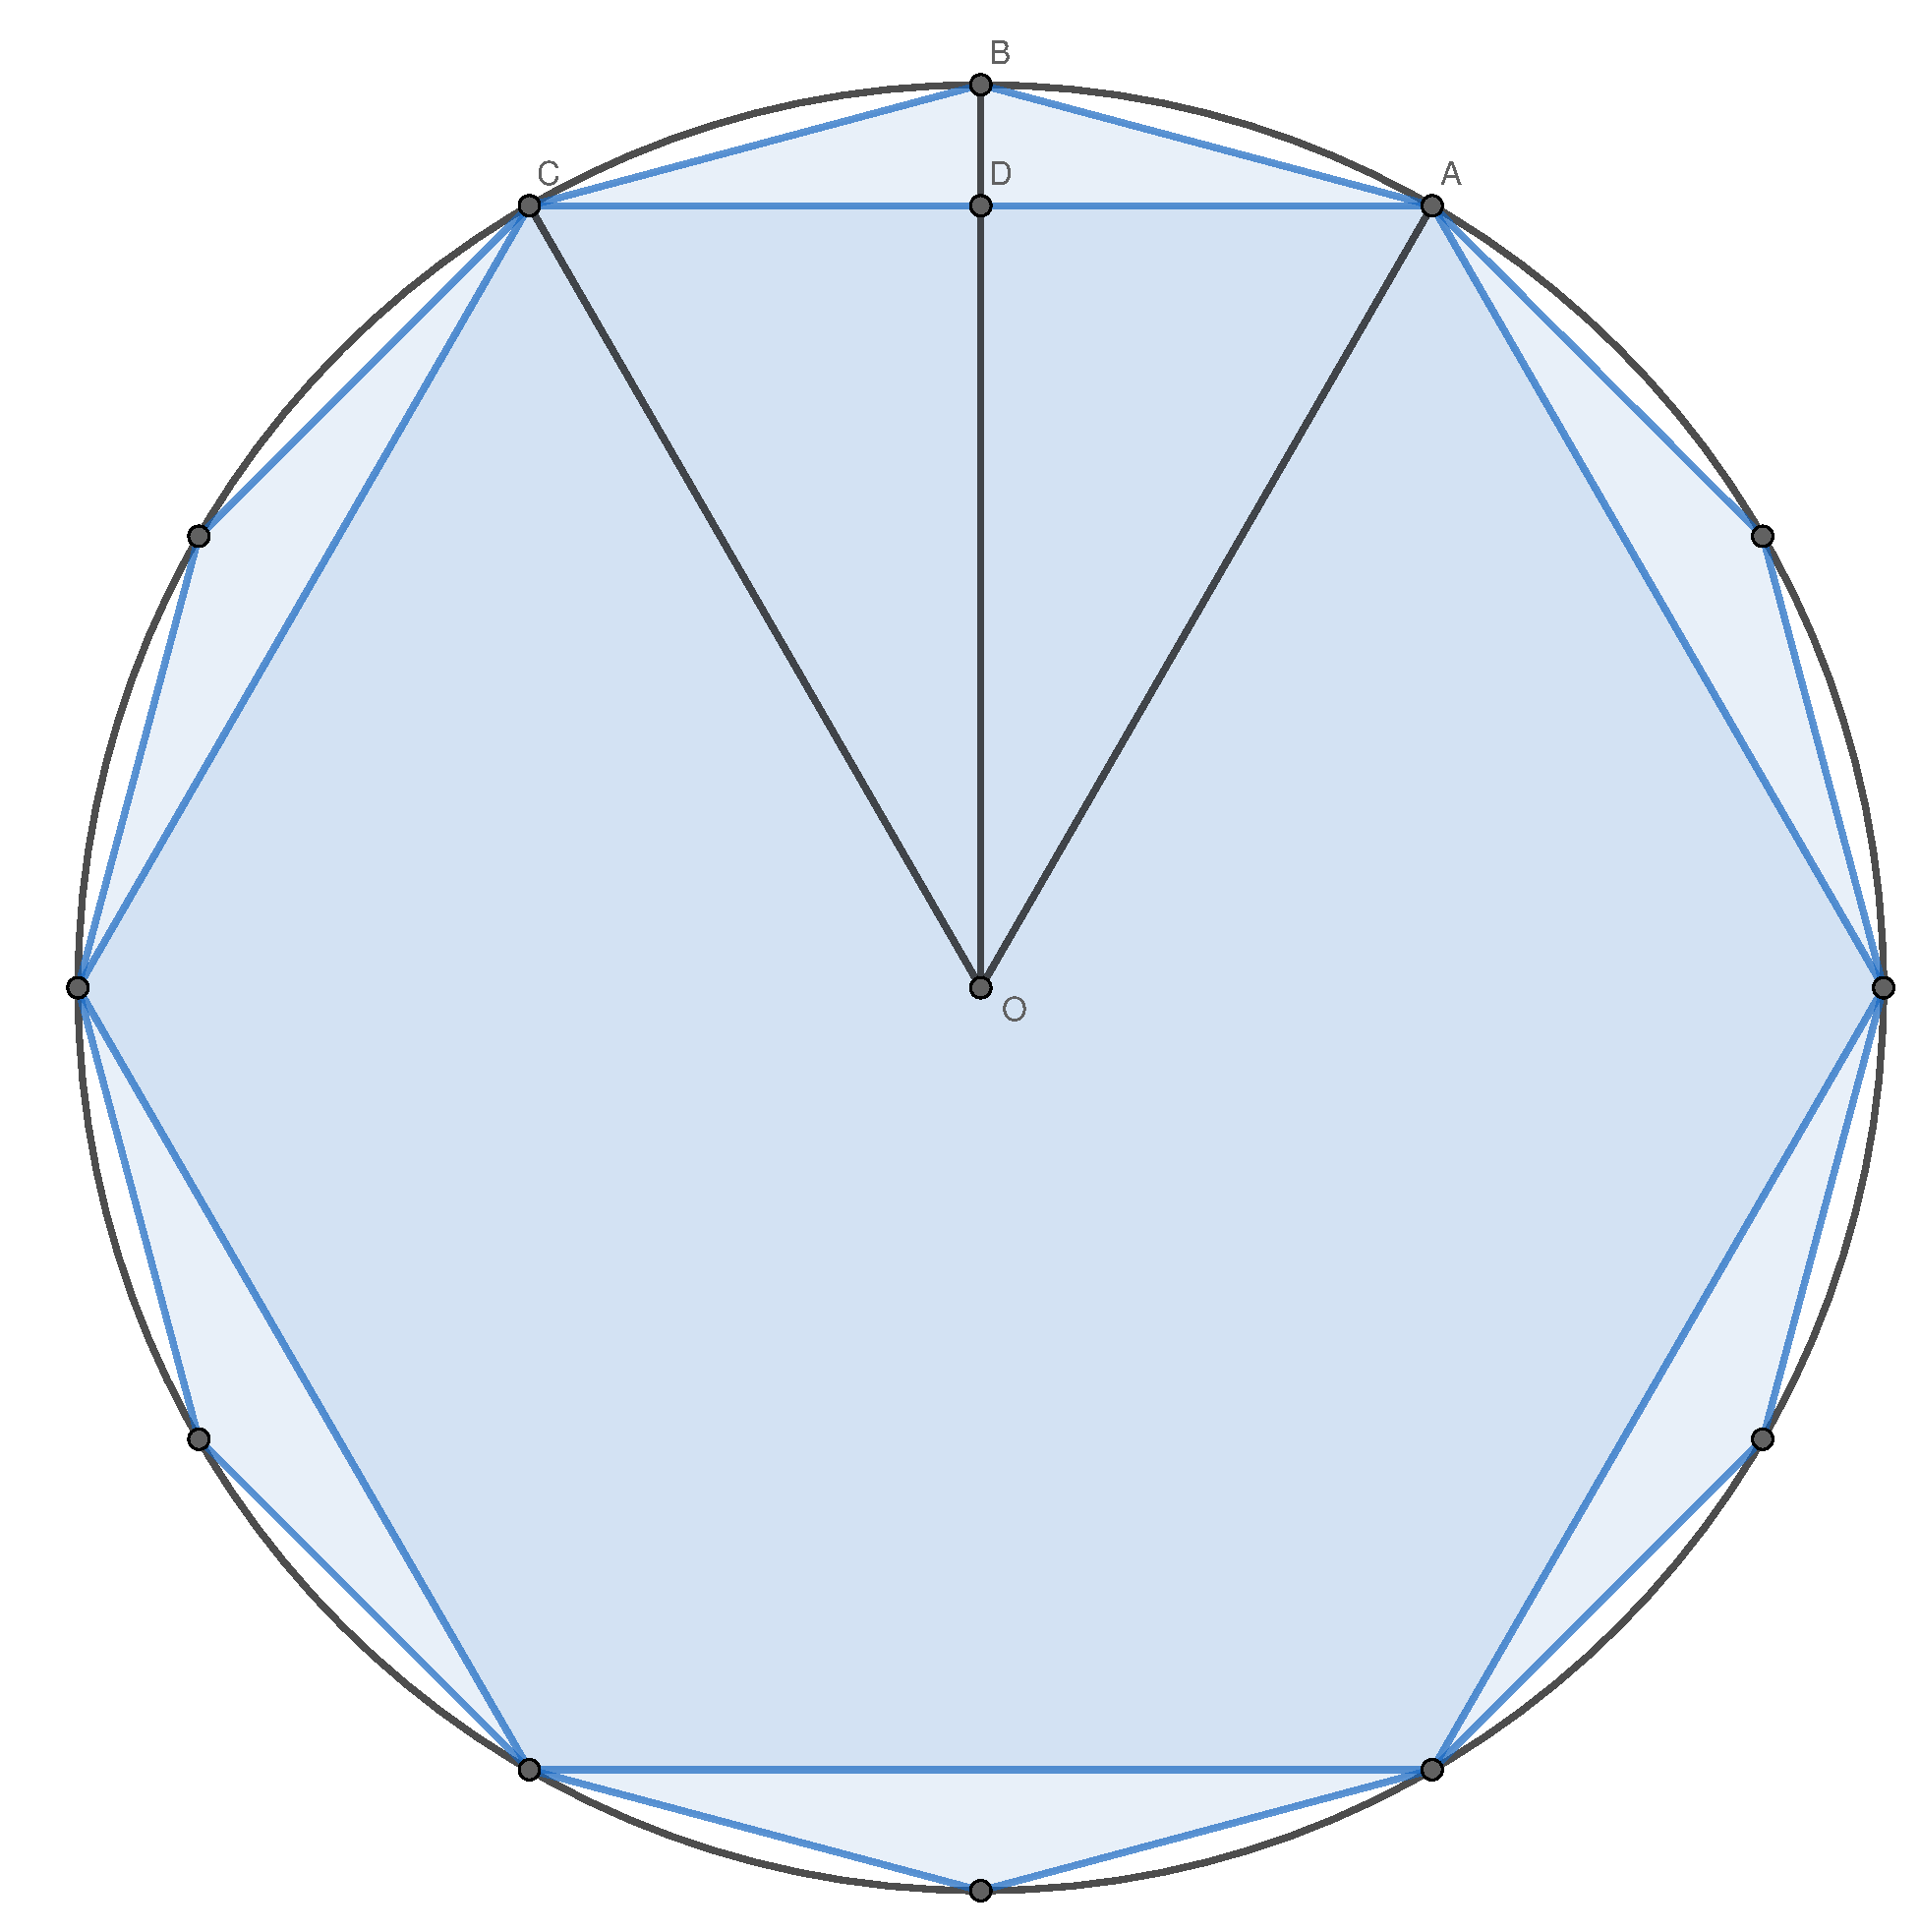
\includegraphics[width=0.7\linewidth]{dodecahedron.pdf}
        \end{center}
        We will work out the area of quadrilateral $OABC$ then multiply by 6, taking advantage of the symmetry in the situation.

        As we showed in class, triangle $\triangle OAC$ is equilateral, because $OA=OC=1$ and $\angle AOC=60^\circ$. Hence the area of $\triangle OAC$ is $\frac{\sqrt 3}4$ (we did this in class). Now we just need to figure out the area of $\triangle ABC$. Its base $AC$ is 1, because it is part of an equilaterial triangle of side length 1; therefore we just need to figure out the height $BD$. But we know that $OB=1$ since $OB$ is a radius, and we can use the Pythagorean theorem on the 30-60-90 triangle $\triangle OAD$ to determine that $OD=\frac{\sqrt 3}2$. Therefore,
        \[BD=OB-OD=1-\frac{\sqrt 3}2=\frac{2-\sqrt3}2,\]
        so the area of $\triangle ABC$ is
        \[\frac 12\cdot 1\cdot \frac{2-\sqrt3}2=\frac{2-\sqrt3}4.\]
        Therefore, the area of quadrilateral $OABC$ is the sum of the area of $\triangle OAB$ and the area of $\triangle ABC$, which is
        \[\frac{\sqrt3}4+\frac{2-\sqrt3}4=\frac12.\]
        Therefore the area of the dodecagon is $6\cdot\frac12=3$. This is pretty close to $\pi$, only about 0.14 off!
    \end{solution}

    \begin{problem}
        Use the method of Riemann sums with 20 equal divisions to approximate $\pi$, using the function $f(x)=\sqrt{1-x^2}$. Use a calculator or computer to help you with all the additions! (Excel or Google Sheets should be helpful here.)
    \end{problem}
    \begin{solution}
        Here is a screenshot of the Riemann sum I worked out in Excel (here I used a left Riemann sum):
        \begin{center}
        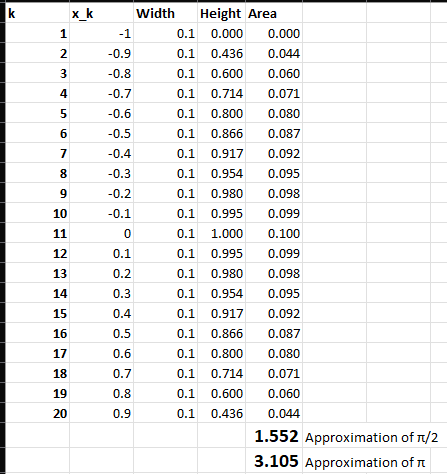
\includegraphics[width=0.5\linewidth]{riemann_sum.png}
        \end{center}
    \end{solution}

    \begin{problem}
        Find a general (possibly piecewise) expression for
        \[\int_a^b |x|\,dx\]
        in terms of the two real numbers $a,b$ (which can each 
        be positive, negative, or zero!).
    \end{problem}
    \begin{solution}
        The definition of the definite integral of $|x|$ with respect to $x$ from $a$ to $b$ is the signed area under the graph of $|x|$ from $a$ to $b$. For example, if $a=7$ and $b=9$, the definite integral would evaluate to the signed area under the graph of $|x|$ from 7 to 9. This can be found by taking a difference of the areas of two isosceles right triangles of leg lengths 9 and 7, respectively. The task at hand is to generalize this computation to any values of $a$ and $b$.

        If $a,b\geq 0$, then the area under the absolute value curve from $a$ to $b$ is equal to $\frac 12(b^2-a^2)$.

        If $b\geq 0$ and $a\leq 0$, then the area is equal to $\frac12(b^2+a^2)$.

        If $b\leq 0$ and $a\geq 0$, then the area is equal to $-\frac12(b^2+a^2)$.

        If $a,b\leq 0$, then the area is equal to $\frac 12(a^2-b^2)$.

        Summing up,
        \[\int_a^b|x|\,dx = \begin{cases}\frac 12(b^2-a^2)& a,b\geq 0\\
            \frac 12(b^2+a^2)& b\geq 0,a\leq 0,\\
            -\frac12(b^2+a^2) &b\leq 0,a\geq 0,\\
            \frac 12(a^2-b^2) &a,b\leq 0.
        \end{cases}\]
        If you were clever and were able to notice that $\frac12 x|x|$ is an antiderivative of $|x|$, then there is a simple expression which is equivalent to the piecewise result with 4 cases: it is $\frac 12(b|b|-a|a|)$! Of course this uses the Fundamental Theorem of Calculus part 2 which has not been covered yet at this point.
    \end{solution}

    \begin{problem}
        For any sequence $\underline a=(a_1,a_2,a_3,\dots)$ of real numbers, define the \emph{finite difference operator} $\Delta$ by 
        \[\Delta(\underline a)=(a_2-a_1,a_3-a_2,a_4-a_3,\dots).\]
        For example, $\Delta(1,2,3,4,\dots)=(1,1,1,1,\dots)$. Also define the \emph{cumulative sum operator} $\Sigma$ by
        \[\Sigma(\underline a)=(a_1,a_1+a_2,a_1+a_2+a_3,\dots).\]
        For example, $\Sigma(1,2,3,4,\dots)=(1,3,6,10,\dots)$. In general, what is $\Delta(\Sigma(\underline a))$? (If you aren't sure, try on a few examples of your own.) Once you find a result, give a proof that your result holds.

        Remark: This is the discrete analog of the fundamental theorem of calculus! Finite differences are the discrete version of derivatives, and cumulative sums are the discrete version of integrals.
    \end{problem}
    \begin{solution}
        Let us directly apply the definitions inside-out: we have by definition
        \[\Sigma(\underline a)=(a_1,a_1+a_2,a_1+a_2+a_3,\dots).\]
        So
        \begin{align*}
            \Delta(\Sigma(\underline a)) &= ((a_1+a_2)-a_1, (a_1+a_2+a_3)-(a_1+a_2),\dots)\\
            &= (a_2,a_3,a_4,\dots).
        \end{align*}
        So $\Delta(\Sigma(\underline a))$ is the so-called shift operator! It deletes the first term and moves all the other terms to the left by one.

        \emph{Remark}: It turns out that if we slightly modify the cumulative sum operator to return $(0,a_1,a_1+a_2,\dots)$ (the difference is that there is a 0 added to the front), then $\Delta(\Sigma(\underline a))$ would be $\underline a$ again, just like in the fundamental theorem of calculus. I should probably change it to this next time I run this class.
    \end{solution}

\end{document}
